\chapter{Einleitung}

\paragraph{Was ist der \ac{ewm-sim}?}
In der vierten industriellen Revolution verändert sich auch der Arbeitsalltag in Lagerhallen.
Mobile Roboter finden verstärkt Einsatz, um die Arbeiter zu unterstützen.
Das Projekt \enquote{\ac{EWM} Cloud Robotics} der SAP hat das Ziel, die Integration von Robotern verschiedenster Hersteller in ein Netzwerk auf Basis von Google Cloud Robotics zu ermöglichen und dieses an ein SAP \ac{EWM}-System anzubinden.
Zu Demonstrations- und Entwicklungszwecken wird eine Simlationsumgebung erstellt, in der ein virtuelles Warenlager präsentiert wird, in dem Roboter beispielhafte Aufträge bearbeiten.
Um nun zu vermeiden, dass ein vollständiges \ac{EWM}-System für solch eine Simulation deployed werden muss, wurde der \enquote{\ac{ewm-sim}} eingeführt.
Er stellt einen kleinen Webserver dar, welcher die Schnittstelle, über die die Roboter ihre Aufträge vom \ac{EWM}-System erhalten, detailgetreu nachbildet.

\paragraph{Kritikpunkte an der ursprünglichen Implementierung}
Wie bereits erwähnt, soll der \ac{ewm-sim} die Schnittstelle eines \ac{EWM}-Systems nachbilden. Hierbei handelt es sich um einen \ac{OData}-Service.
Für die Implementierung wurde hier auf den bestehenden Mock Server von SAPUI5 gesetzt, der normalerweise in der Frontendentwicklung dazu dient, entsprechende Schnittstellen einer Datenbank nachzubilden.
Dieser ist jedoch nicht für die Backend-Entwicklung vorgesehen.
Leider bringt er somit das Problem mit sich, dass er sich nur innerhalb der Laufzeitumgebung einer SAPUI5-App verwenden lässt, welche wiederum zwangsläufig in einem Browser laufen muss.
In der \autoref{fig:ewm-sim-v1} ist der Aufbau des bisherigen \ac{ewm-sim} veranschaulicht.
Er stellt eine Art gekapseltes System dar.
Die Anfragen, die an den nach außen hin geöffneten Webserver geschickt werden, landen über den WebSocket Server bei einer headless Instanz von Google Chrome, in welchem wiederum eine SAPUI5-App ausgeführt wird.
Diese ist mit dem SAPUI5 Mock Server verknüpft, welcher die Daten, die er bereitstellen soll, aus einer \code{\ac{JSON}}-Datei einliest.

Wie gut zu erkennen ist, bringt diese Implementierung einen großen Overhead und somit mögliche Fehlerquellen mit sich. Ziel des in dieser Praxisarbeit behandelten Projekts soll es sein, das Konzept des \ac{ewm-sim} zu optimieren und diesen daraufhin im Anschluss neu zu implementieren.

\begin{figure}
    \centering
    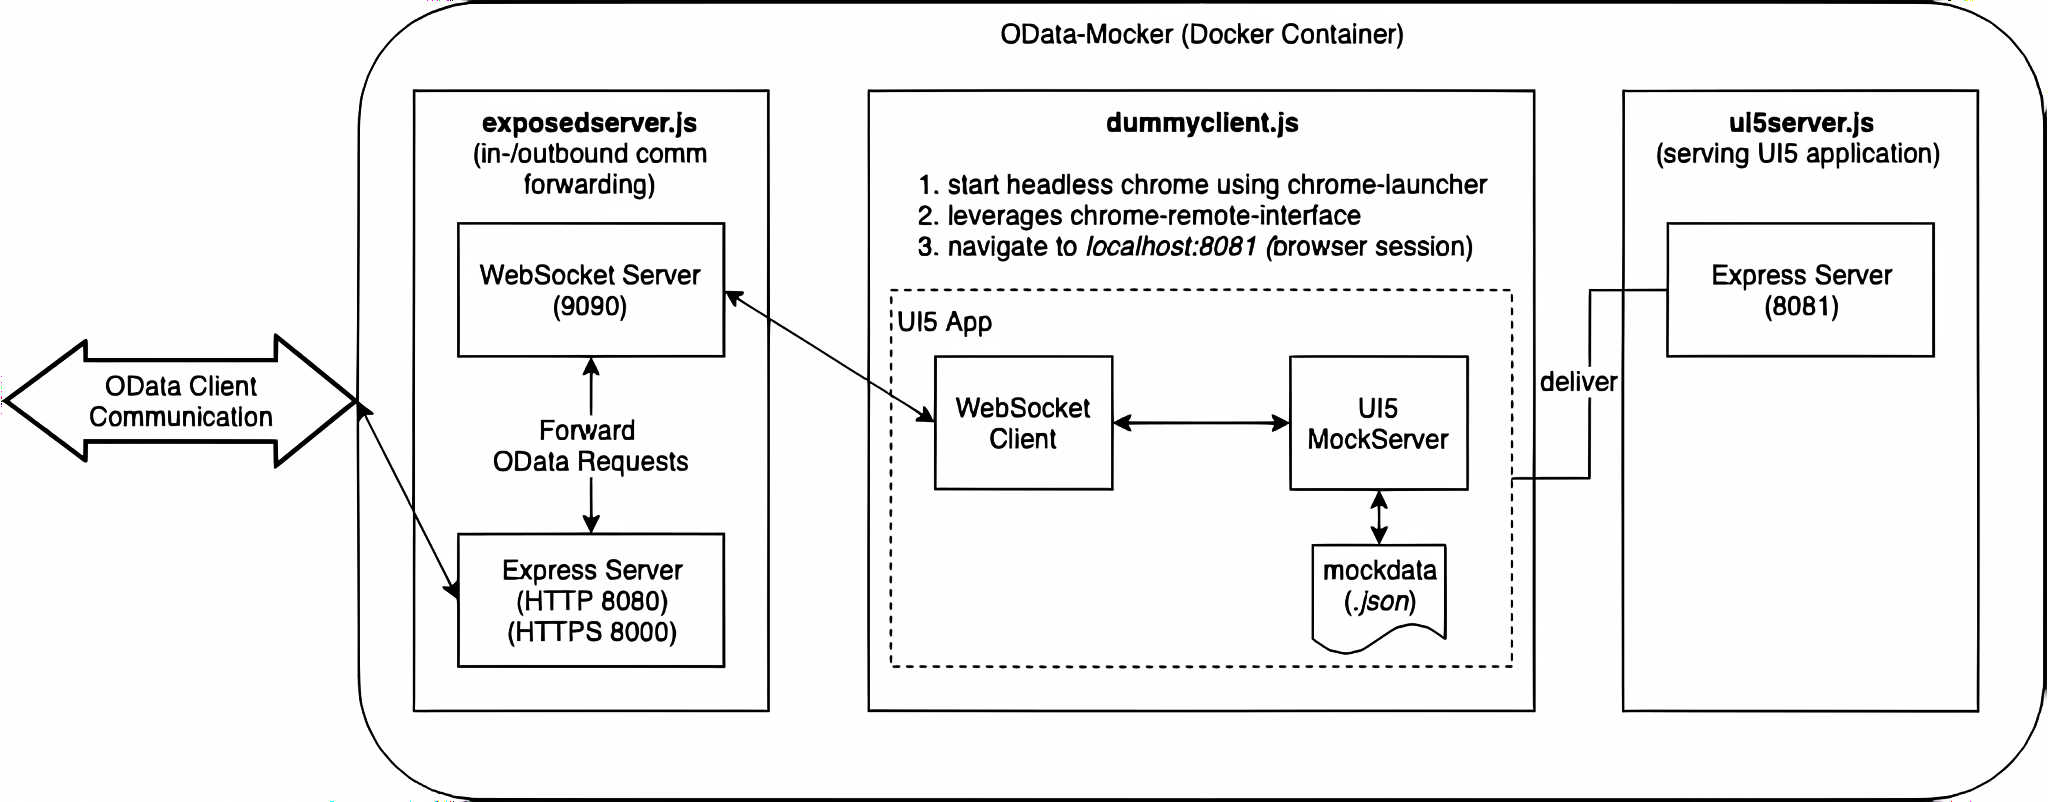
\includegraphics[width=\textwidth]{Bilder/ewm-sim_v1_4x.pdf}
    \caption{Aufbau des ursprünglichen \ac{ewm-sim}}
    \label{fig:ewm-sim-v1}
\end{figure}

% \todo{Verweis auf Studentenprojekt, Zusammenarbeit mit Roboter-Anbindung und Unity Simulation}